%
%===============>>  ГРУППА 10-2 МОДУЛЬ 6  <<=============
%
\setmodule{6}

%BEGIN_FOLD % ====>>_____ Занятие 1 _____<<====
\begin{class}[number=1]
	\begin{listofex}
		\item Вычислите:
		\begin{tasks}(4)
			\task \( \sqrt[4]{16} \)
			\task \( \sqrt[5]{243} \)
			\task \( \sqrt[3]{64} \)
			\task \( \sqrt[3]{-27} \)
			\task \( \sqrt[4]{64} \)
			\task \( \sqrt[5]{-64} \)
			\task \( \sqrt[3]{0,125} \)
			\task \( \sqrt[7]{-128} \)
		\end{tasks}
		\item Извлеките корень:
		\begin{tasks}(4)
			\task \( \sqrt[3]{a^6b^9} \)
			\task \( \sqrt[3]{64x^3z^6} \)
			\task \( \sqrt[3]{a^{12}b^3} \)
			\task \( \sqrt[3]{1000a^6b^6} \)
		\end{tasks}
		\item Найдите произведение:
		\begin{tasks}(2)
			\task \( \sqrt[3]{ab^2} \cdot \sqrt[3]{a^2b} \)
			\task \( \sqrt[3]{a^2b^4} \cdot \sqrt[3]{ab^2} \)
			\task \( \sqrt[3]{3,7^4} \cdot \sqrt[4]{3,7^3} : \sqrt[12]{3,7} \)
			\task \( \sqrt[4]{2,5^3} : \sqrt[12]{2,5} \cdot \sqrt[3]{2,5^4} \)
		\end{tasks}
		\item Вычислите:
		\begin{tasks}(3)
			\task \( \sqrt[3]{27 \cdot 0,001 \cdot 125} \)
			\task \( \sqrt[4]{625 \cdot 0,0016 \cdot 256} \)
			\task \( \sqrt[5]{243 \cdot 0,00001 \cdot 0,00032} \)
		\end{tasks}
		\item Вынесите множитель из под знака корня:
		\begin{tasks}(4)
			\task \( \sqrt[3]{40} \)
			\task \( \sqrt[5]{-64} \)
			\task \( \sqrt[5]{-96} \)
			\task \( \sqrt[3]{54} \)
		\end{tasks}
		\item Вычислите:
		\begin{tasks}(2)
			\task \( \sqrt[3]{125 \cdot 27} \)
			\task \( \sqrt[4]{16 \cdot 625} \)
			\task \( \sqrt[4]{81 \cdot 16} \)
			\task \( \sqrt[4]{5 \cdot 125} \)
			\task \( \sqrt[3]{\dfrac{1}{64}} +\sqrt[4]{\dfrac{81}{64}} - \sqrt[5]{\dfrac{1}{32}} \)
			\task \( \dfrac{\sqrt[]{3}}{\sqrt[]{27}} - \dfrac{\sqrt[]{125}}{\sqrt[]{5}} \)
			\task \( \dfrac{\sqrt[]{5}}{\sqrt[]{125}} - \dfrac{\sqrt[]{343}}{\sqrt[]{7}} \)
			\task \( \sqrt[]{0,0016} : \sqrt[4]{0,0016} \)
		\end{tasks}
		\item Решите уравнения:
		\begin{tasks}(2)
			\task \( \sqrt[3]{15-2x} = 3 \)
			\task \( \sqrt[4]{2x-8}=3 \)
			\task \( \sqrt[3]{4x^2-5x-1}=2 \)
			\task \( \sqrt[]{-72-17x}=-x \)
			\task \( \sqrt[]{\dfrac{1}{1-5x}}=\dfrac{1}{6} \)
			\task \( \sqrt[3]{\dfrac{128}{x^2-2x+3}}=4 \)
		\end{tasks}
		\item Из пункта \(A\) в пункт \(B\) одновременно выехали два автомобиля. Первый проехал с постоянной скоростью весь путь. Второй проехал первую половину пути со скоростью, меньшей скорости первого на \(13\) км/ч, а вторую половину пути  --- со скоростью \(78\) км/ч, в результате чего прибыл в пункт \(B\) одновременно с первым автомобилем. Найдите скорость первого автомобиля, если известно, что она больше \(48\) км/ч. Ответ дайте в км/ч.
	\end{listofex}
\end{class}
%END_FOLD

%BEGIN_FOLD % ====>>_____ Занятие 2 _____<<====
\begin{class}[number=2]
	\begin{listofex}
		\item Вычислите:
		\begin{tasks}(4)
			\task \( \sqrt[3]{512} \)
			\task \( \sqrt[7]{128} \)
			\task \( \sqrt[5]{1024} \)
			\task \( \sqrt[4]{81} \)
		\end{tasks}
		\item Вычислите:
		\begin{tasks}(3)
			\task \( \sqrt[3]{1000 \cdot 512} \)
			\task \( \sqrt[3]{343 \cdot 0,125} \)
			\task \( \sqrt[4]{1296 \cdot 0,0001 \cdot 1024} \)
		\end{tasks}
		\item Извлеките корень из дроби:
		\begin{tasks}(3)
			\task \( \sqrt[3]{\dfrac{1}{64}} \)
			\task \( \sqrt[4]{\dfrac{81}{16}} \)
			\task \( \sqrt[5]{\dfrac{32}{243}} \)
		\end{tasks}
		\item Вынесите множитель из под знака корня:
		\begin{tasks}(4)
			\task \( \sqrt[3]{\dfrac{3}{8}} \)
			\task \( \sqrt[3]{\dfrac{27}{4}} \)
			\task \( \sqrt[3]{-\dfrac{250}{16}} \)
			\task \( \sqrt[3]{-\dfrac{64}{7}} \)
		\end{tasks}
		\item Вычислите:
		\begin{tasks}(4)
			\task \( \sqrt[]{(-2)^2} \)
			\task \( \sqrt[]{(-5)^4} \)
			\task \( \sqrt[]{(\sqrt{2}-1)^2} \)
			\task \( \sqrt[]{(\sqrt{2}-2)^2} \)
		\end{tasks}
		\item Упростите выражение:
		\begin{tasks}(2)
			\task \( \sqrt[4]{81 \cdot (4-\sqrt{17})^4} \)
			\task \( \sqrt[3]{0,001} - \sqrt[6]{0,000064} \)
		\end{tasks}
		\item Вычислите:
		\begin{tasks}(1)
			\task \( \sqrt[3]{343} - \sqrt{4,84}+ \sqrt[5]{0,00032} \)
			\task \( \sqrt[3]{256} + \sqrt[6]{9^3} - \sqrt[10]{32^2} \)
			\task \( \sqrt[20]{0,25} : \sqrt[4]{0,25^5} : \sqrt[5]{0,25^4} \)
		\end{tasks}
		\item Извлеките корень:
		\begin{tasks}(3)
			\task \( \sqrt[]{ 81a^2b^8 } \)
			\task \( \sqrt[]{ 25a^6b^4 } \)
			\task \( \sqrt[3]{ 8a^3b^6 } \)
			\task \( \sqrt[3]{ 0,001a^6b^{12} } \)
			\task \( \sqrt[4]{ 1000a^4b^{16} } \)
			\task \( \sqrt[4]{ 81a^8b^{12}} \)
		\end{tasks}
		\item Решите уравнения:
		\begin{tasks}(2)
			\task \( \sqrt[3]{6+5x} = x \)
			\task \( \sqrt[]{x-2}=6 \)
			\task \( \sqrt[4]{4x-5}=2 \)
			\task \( \sqrt[]{-4-5x}=x \)
			\task \( \sqrt[]{\dfrac{1}{15-4x}}=0,2 \)
			\task \( \sqrt[3]{\dfrac{27}{-2x^2-6x+1}}=3 \)
		\end{tasks}
		\item Из пункта \(A\) в пункт \(B\), расстояние между которыми \(75\) км, одновременно выехали автомобилист и велосипедист. Известно, что за час автомобилист проезжает на \(40\) км больше, чем велосипедист. Определите скорость велосипедиста, если известно, что он прибыл в пункт \(B\) на \(6\) часов позже автомобилиста. Ответ дайте в км/ч.
	\end{listofex}
\end{class}
%END_FOLD

%BEGIN_FOLD % ====>>_ Домашняя работа 1 _<<====
\begin{homework}[number=1]
	\begin{listofex}
		\item Вычислите:
		\begin{tasks}(4)
			\task \( \sqrt[3]{343} \)
			\task \( \sqrt[4]{625} \)
			\task \( \sqrt[5]{32} \)
			\task \( \sqrt[4]{1296} \)
		\end{tasks}
		\item Извлеките корень из дроби:
		\begin{tasks}(3)
			\task \( \sqrt[3]{\dfrac{125}{216}} \)
			\task \( \sqrt[4]{\dfrac{625}{16}} \)
			\task \( \sqrt[3]{\dfrac{512}{27}} \)
		\end{tasks}
		\item Извлеките корень:
		\begin{tasks}(3)
			\task \( \sqrt[]{ 25a^4b^6 } \)
			\task \( \sqrt[3]{ 27a^6b^9 } \)
			\task \( \sqrt[5]{ 1024a^{15}b^{20} } \)
		\end{tasks}
		\item Вычислите:
		\begin{tasks}(2)
			\task \( \sqrt[]{(\sqrt{2}-\sqrt{3})^2} \)
			\task \( \dfrac{(\sqrt{7}-\sqrt{6})^3(\sqrt{7}+\sqrt{6})^3}{0,125} \)
		\end{tasks}
		\item Вычислите:
		\begin{tasks}(3)
			\task \( (\sqrt[3]{-2})^3 + (\sqrt[5]{8})^5 \)
			\task \( \sqrt[5]{-1} + \sqrt[3]{-8} \)
			\task \( \sqrt[5]{8} \cdot \sqrt[5]{4} \)
			\task \( \sqrt[3]{4} \cdot \sqrt[3]{8} \cdot \sqrt[3]{-2} \)
			\task \( \sqrt[3]{1,8} \cdot \sqrt[3]{0,12} \)
			\task \( \sqrt[4]{0,54} \cdot \sqrt[4]{0,24} \)
		\end{tasks}
		\item Решите уравнения:
		\begin{tasks}(2)
			\task \( \sqrt[]{4x+4} = x-2 \)
			\task \( \sqrt[3]{x^2+4x-4}=2 \)
		\end{tasks}
		\item 
		\begin{minipage}[t]{\bodywidth}
			На рисунке изображен график функции вида \( f(x)=\dfrac{x^2}{a}+bx+c \), где \( a, b, c \) --- целые числа. Найдите значение: \( f(7) \)
		\end{minipage}
		\hspace{0.02\linewidth}
		\begin{minipage}[t]{\picwidth}
			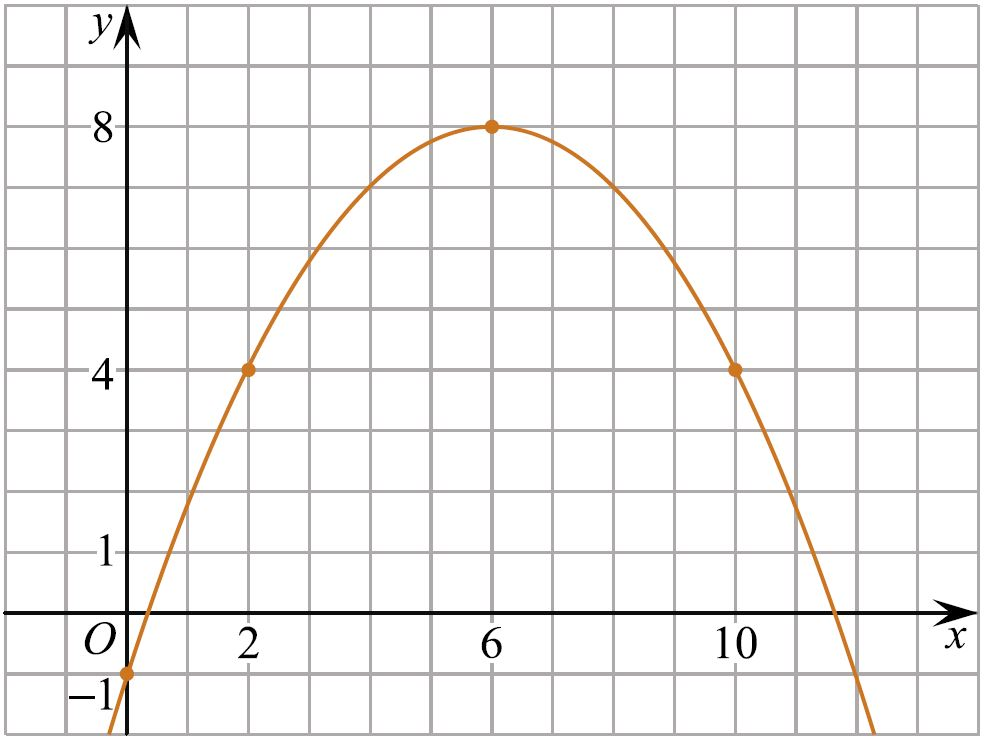
\includegraphics[align=t, width=\linewidth]{\picpath/G112M3C2-3}
		\end{minipage}
		\item Из пункта \(A\) в пункт \(B\) одновременно выехали два автомобиля. Первый проехал с постоянной скоростью весь путь. Второй проехал первую половину пути со скоростью \(24\) км/ч, а вторую половину пути --- со скоростью, на \(16\) км/ч большей скорости первого, в результате чего прибыл в пункт \(B\) одновременно с первым автомобилем. Найдите скорость первого автомобиля. Ответ дайте в км/ч.
	\end{listofex}
\end{homework}
%END_FOLD

%BEGIN_FOLD % ====>>_____ Занятие 3 _____<<====
\begin{class}[number=3]
	\begin{listofex}
		\item Занятие 3 
	\end{listofex}
\end{class}
%END_FOLD

%BEGIN_FOLD % ====>>_____ Занятие 4 _____<<====
\begin{class}[number=4]
	\begin{listofex}
		\item Занятие 4
	\end{listofex}
\end{class}
%END_FOLD

%BEGIN_FOLD % ====>>_ Домашняя работа 2 _<<====
\begin{homework}[number=2]
	\begin{listofex}
		\item Домашняя работа 2
	\end{listofex}
\end{homework}
%END_FOLD

%BEGIN_FOLD % ====>>_____ Занятие 5 _____<<====
\begin{class}[number=5]
	\begin{listofex}
		\item Занятие 5
	\end{listofex}
\end{class}
%END_FOLD
	
%BEGIN_FOLD % ====>>_____ Занятие 6 _____<<====
\begin{class}[number=6]
	\begin{listofex}
		\item Занятие 6
	\end{listofex}
\end{class}
%END_FOLD
	
%BEGIN_FOLD % ====>>_ Домашняя работа 3 _<<====
\begin{homework}[number=3]
	\begin{listofex}
		\item Домашняя работа 3
	\end{listofex}
\end{homework}
%END_FOLD
	
%BEGIN_FOLD % ====>>_____ Занятие 7 _____<<====
\begin{class}[number=7]
	\title{Подготовка к проверочной}
	\begin{listofex}
		\item Занятие 7
	\end{listofex}
\end{class}
%END_FOLD
	
%BEGIN_FOLD % ====>>_ Проверочная работа _<<====
\begin{exam}
	\begin{listofex}
		\item Проверочная
	\end{listofex}
\end{exam}
%END_FOLD